\documentclass[./main.tex]{subfiles}

\begin{document}
\chapter*{the process of human learning}

The word `human' is important, as mathematics, science, philosophy etc... are after all, human made things and there is nothing `absolute' or `exact' about them.
So, there is no reason to be serious or stuck up with anything (especially science).
Beliefs lies at the heart of all human made things (even science and the mighty math).
As beliefs are not unconditionally correct, nothing should be blindly accepted forever, rather everything better be constantly challenged.
This does not mean that nothing should be trusted, that might be even worse.

It is in the \textbf{balance} between having trust and challenging it simultaneously lies any \textbf{conceivable progress}.
If the balance tips left it is called `arrogance', else if it tips right it is called `insanity'.
If the balance is right it produces a sense of happiness, fun and joy.
\textbf{In fact finding this joy through the balance is the spirit of science itself.}.

I believe that this feeling is what human beings pursuing science crave for.
Also, I personally have an application-oriented mindset, as in if I can apply my knowledge to create/improve a tangible system, it produces a great sense of joy to me.
So I guess if I bring some kind of application to every piece of new thing I learn then I might have a deeper (a more intimate) insight in it.

\begin{figure}[h]
  \centering
  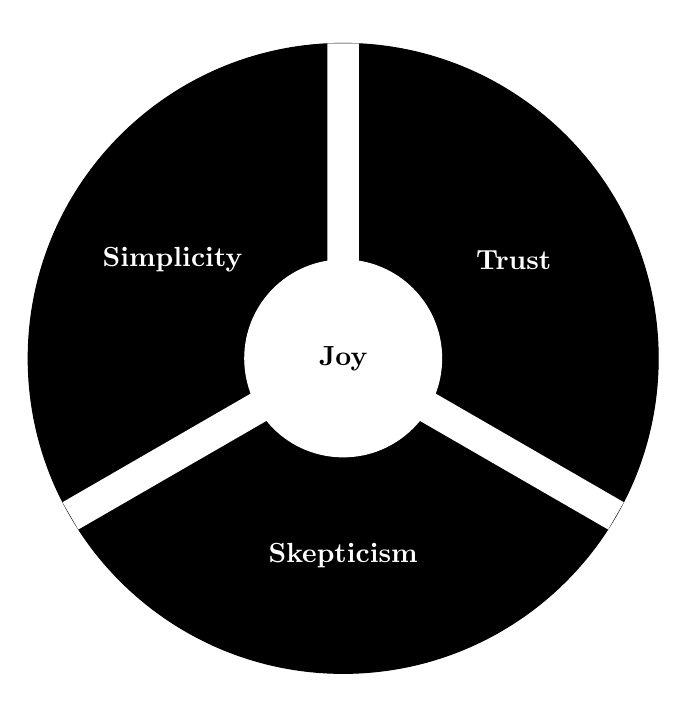
\begin{tikzpicture}
    \draw[fill=black] (0,0) circle (4);
    \draw[line width=4mm, white] (0,4) -- (0,0) -- (4*0.866,-4*0.5) (0,0) -- (-4*0.866,-4*0.5);
    \node[white] at (-2.5*0.866,2.5*0.5) {\textbf{Simplicity}};
    \node[white] at (2.5*0.866,2.5*0.5) {\textbf{Trust}};
    \node[white] at (0,-2.5) {\textbf{Skepticism}};
    \draw[white, fill=white] (0,0) circle (1.25) node {\textbf{{\color{black} Joy}}};
  \end{tikzpicture}
  \label{fig:human_learning}
  \caption{Zen of human learning}
\end{figure}

\end{document}

